\documentclass[tikz, border=5pt]{standalone}

\usepackage{tikz}
\usetikzlibrary{
  arrows.meta,
  calc,
  positioning,
  shapes.geometric,
  shadows.blur,
  bending
}

\begin{document}

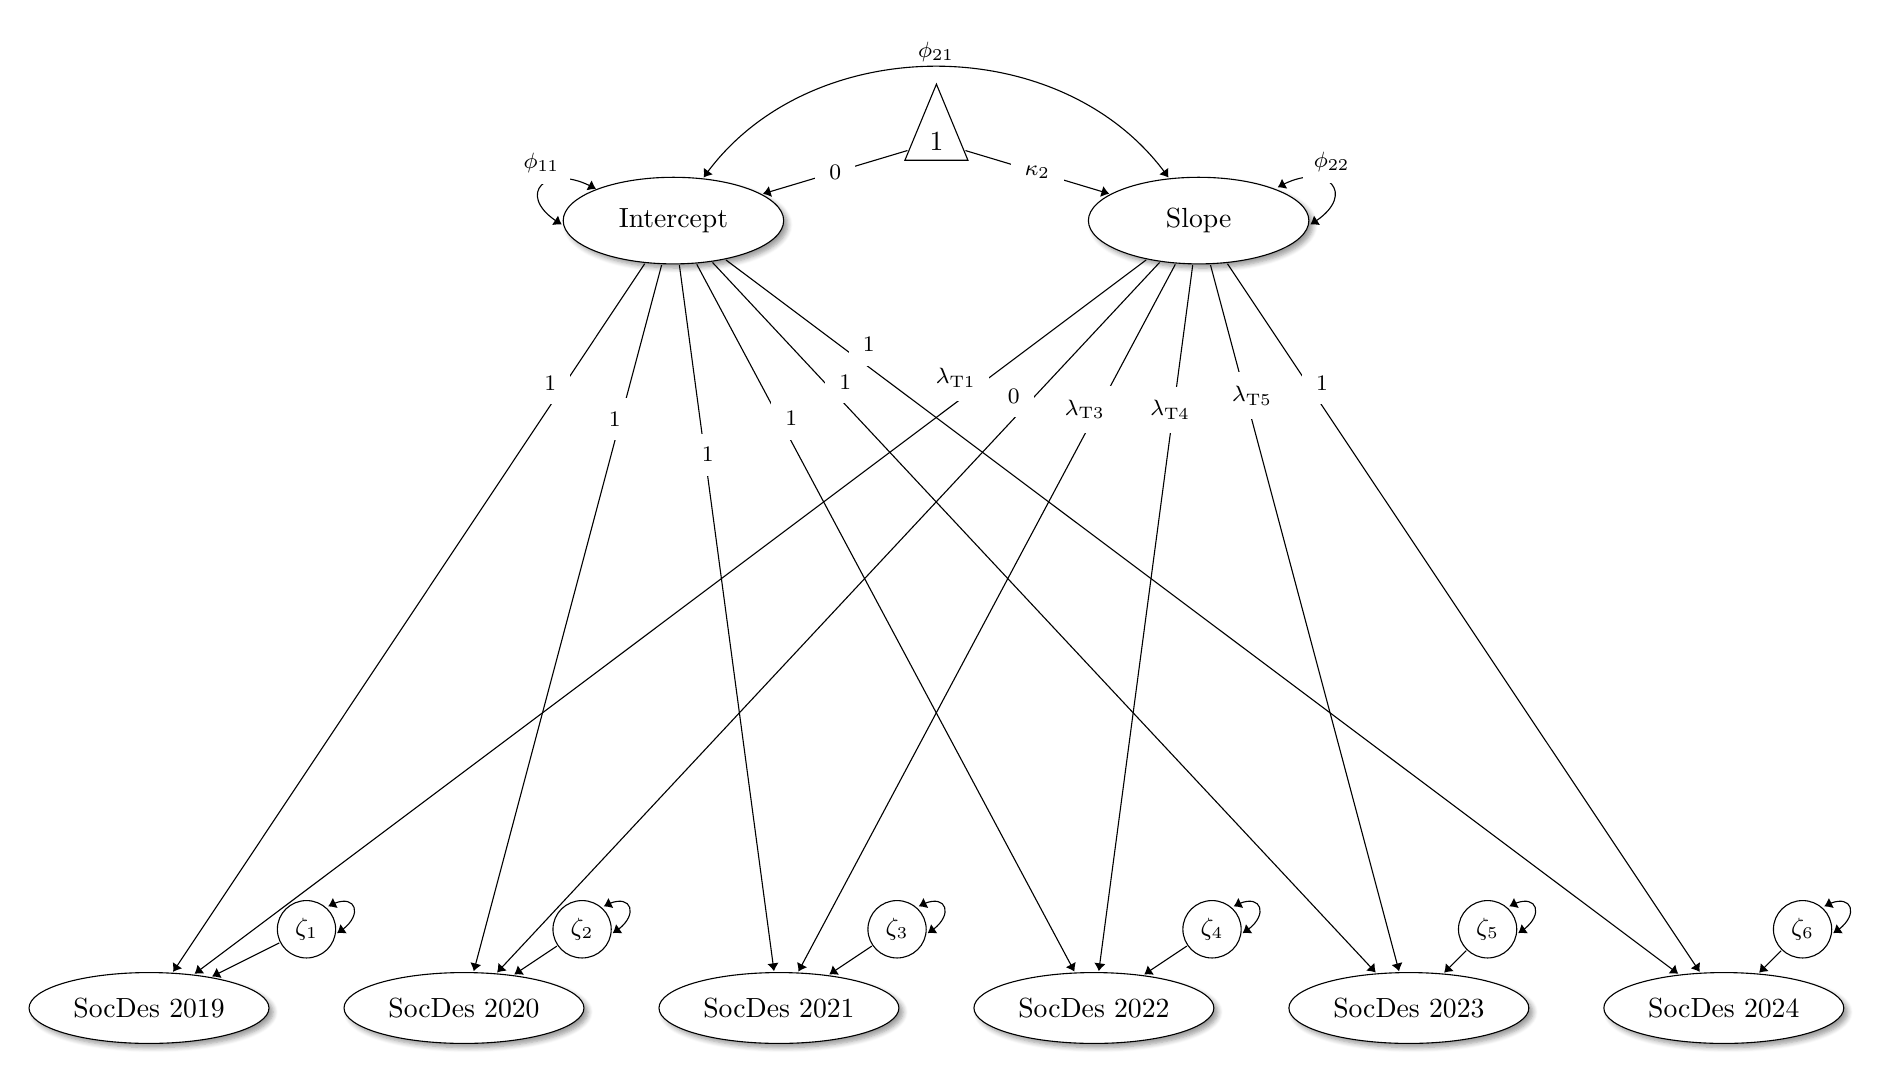
\begin{tikzpicture}

\tikzset{
  socdes/.style={
    draw,
    ellipse,
    fill=white,
    minimum width=2.6cm,
    minimum height=0.9cm,
    align=center,
    blur shadow={shadow xshift=1.5pt, shadow yshift=-1.5pt, shadow blur steps=6}
  },
  latent/.style={
    draw,
    ellipse,
    fill=white,
    minimum width=2.8cm,
    minimum height=1.1cm,
    align=center,
    blur shadow={shadow xshift=1.5pt, shadow yshift=-1.5pt, shadow blur steps=6}
  },
  >={Latex[length=1mm, width=1.5mm]},
  line width=1pt
}

% Noded SocDes
\node[socdes] (y1) at (0,  0) {SocDes 2019};
\node[socdes] (y2) at (4,  0) {SocDes 2020};
\node[socdes] (y3) at (8,  0) {SocDes 2021};
\node[socdes] (y4) at (12, 0) {SocDes 2022};
\node[socdes] (y5) at (16, 0) {SocDes 2023};
\node[socdes] (y6) at (20, 0) {SocDes 2024};

% Nodes Growth Factors
\node[latent] (I) at (6.66, 10) {Intercept};
\node[latent] (S) at (13.33,10) {Slope};

% Nodes residuals
\node[draw, ellipse, minimum width=0.2cm, minimum height=0.1cm] (z1) at (2,1)    {\small $\zeta_{1}$};
\node[draw, ellipse, minimum width=0.2cm, minimum height=0.1cm] (z2) at (5.5,1)  {\small $\zeta_{2}$};
\node[draw, ellipse, minimum width=0.2cm, minimum height=0.1cm] (z3) at (9.5,1)  {\small $\zeta_{3}$};
\node[draw, ellipse, minimum width=0.2cm, minimum height=0.1cm] (z4) at (13.5,1) {\small $\zeta_{4}$};
\node[draw, ellipse, minimum width=0.2cm, minimum height=0.1cm] (z5) at (17,1)   {\small $\zeta_{5}$};
\node[draw, ellipse, minimum width=0.2cm, minimum height=0.1cm] (z6) at (21,1)   {\small $\zeta_{6}$};

% Node mean
\node[draw, isosceles triangle, shape border rotate=90, minimum size=0.8cm] (const) at (10,11) {1};


% Arrows S
\draw[->] (S) -- node[pos=0.2, above, font=\footnotesize, fill=white, inner sep=5pt] {$\lambda_{\mathrm{T}1}$} (y1);
\draw[->] (S) -- node[pos=0.22, above, font=\footnotesize, fill=white, inner sep=5pt] {0} (y2);
\draw[->] (S) -- node[pos=0.24, above, font=\footnotesize, fill=white, inner sep=5pt] {$\lambda_{\mathrm{T}3}$} (y3);
\draw[->] (S) -- node[pos=0.24, above, font=\footnotesize, fill=white, inner sep=5pt] {$\lambda_{\mathrm{T}4}$} (y4);
\draw[->] (S) -- node[pos=0.22, above, font=\footnotesize, fill=white, inner sep=5pt] {$\lambda_{\mathrm{T}5}$} (y5);
\draw[->] (S) -- node[pos=0.2, above, font=\footnotesize, fill=white, inner sep=5pt] {1} (y6);

% Arrows I
\draw[->] (I) -- node[pos=0.2, above, font=\footnotesize, fill=white, inner sep=5pt] {1} (y1);
\draw[->] (I) -- node[pos=0.25, above, font=\footnotesize, fill=white, inner sep=5pt] {1} (y2);
\draw[->] (I) -- node[pos=0.3, above, font=\footnotesize, fill=white, inner sep=5pt] {1} (y3);
\draw[->] (I) -- node[pos=0.25, above, font=\footnotesize, fill=white, inner sep=5pt] {1} (y4);
\draw[->] (I) -- node[pos=0.20, above, font=\footnotesize, fill=white, inner sep=5pt] {1} (y5);
\draw[->] (I) -- node[pos=0.15, above, font=\footnotesize, fill=white, inner sep=5pt] {1} (y6);

% Arrows Cov I S
\draw[<->] (I) to[bend left=55] node[midway, above, font=\footnotesize, fill=white, inner sep=1pt] {$\phi_{21}$} (S);

% Arrows mean
\draw[->] (const) -- node[pos=0.5, font=\footnotesize, fill=white, inner sep=5pt] {0}          (I);
\draw[->] (const) -- node[pos=0.5, font=\footnotesize, fill=white, inner sep=5pt] {$\kappa_2$} (S);

% Arrows zeta
\draw[->] (z1) -- (y1);
\draw[->] (z2) -- (y2);
\draw[->] (z3) -- (y3);
\draw[->] (z4) -- (y4);
\draw[->] (z5) -- (y5);
\draw[->] (z6) -- (y6);

% Variance of I
\draw[<->]
($(I.north west)+(0.02,0.00)$)
to[out=150, in=150, looseness=3]
node[pos=0.5, above, font=\footnotesize, fill=white, inner sep=4pt] {$\phi_{11}$}
($(I.west)+(0,-0.05)$);

% Variance of S
\draw[<->]
($(S.north east)+(0.00,0.02)$)
to[out=30, in=30, looseness=3]
node[pos=0.5, above, font=\footnotesize, fill=white, inner sep=4pt] {$\phi_{22}$}
($(S.east)+(0,-0.05)$);

% Variances of Zetas
% Variance of zeta 1
\draw[<->]
($(z1.north east)+(0.00,0.02)$)
to[out=30, in=30, looseness=3]
($(z1.east)+(0,-0.05)$);

% Variance of zeta 2
\draw[<->]
($(z2.north east)+(0.00,0.02)$)
to[out=30, in=30, looseness=3]
($(z2.east)+(0,-0.05)$);

% Variance of zeta 3
\draw[<->]
($(z3.north east)+(0.00,0.02)$)
to[out=30, in=30, looseness=3]
($(z3.east)+(0,-0.05)$);

% Variance of zeta 4
\draw[<->]
($(z4.north east)+(0.00,0.02)$)
to[out=30, in=30, looseness=3]
($(z4.east)+(0,-0.05)$);

% Variance of zeta 5
\draw[<->]
($(z5.north east)+(0.00,0.02)$)
to[out=30, in=30, looseness=3]
($(z5.east)+(0,-0.05)$);

% Variance of zeta 6
\draw[<->]
($(z6.north east)+(0.00,0.02)$)
to[out=30, in=30, looseness=3]
($(z6.east)+(0,-0.05)$);

\end{tikzpicture}

\end{document}